Les méthodes agiles proposent une approche flexible et itérative du développement, centrée sur la réduction des risques, l’adaptabilité et la satisfaction du client. Scrum est la méthode agile la plus couramment adoptée\cite{agile}.

Le choix méthodologique retenu pour notre application, défini dès le début du stage, résulte d’une réflexion collective. Il a été guidé par les besoins du projet et la stratégie de l’entreprise, notamment en matière d’approche, de langage de modélisation et de processus de développement.
\subsection{Fonctionnement général de Scrum\cite{Scrum}}
Scrum repose sur des itérations successives "sprints", comme l’illustre la figure \ref{fig:Scrum}, permettant une livraison progressive du produit et visant à apporter de la valeur au client en favorisant la transparence, la collaboration et l’amélioration continue.
\begin{figure}[H]
    \centering
    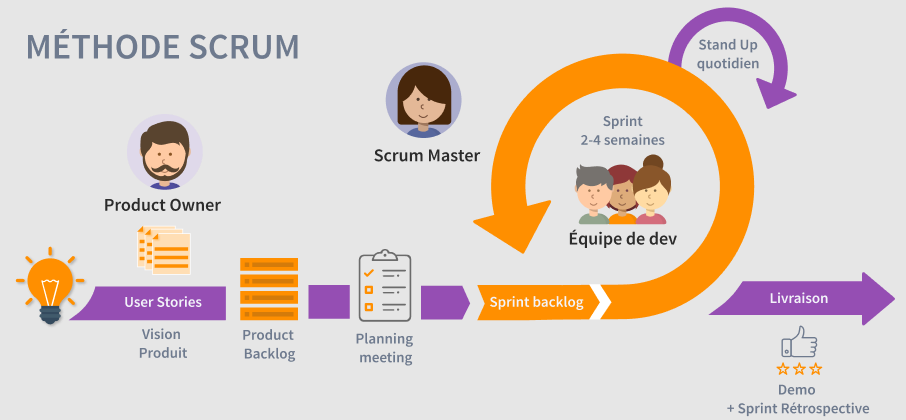
\includegraphics[width=\linewidth]{chapitres/ch1/img/scrum.PNG}
    \caption{Cadre méthodologique et mode de fonctionnement SCRUM \cite{ScrumImg}}
    \label{fig:Scrum}
\end{figure}
\vspace{-0.5cm}
L’équipe Scrum se compose de trois rôles clés:
\begin{itemize}[label=$\bullet$]
    \item \textbf{Product Owner:} Gère le backlog et définit les priorités selon les besoins client.
    \item \textbf{Scrum Master:} Garantit le respect de la méthodologie et facilite le travail de l’équipe.
    \item \textbf{Équipe de développement:} Chargée de la réalisation des fonctionnalités et de la livraison des incréments du produit.
\end{itemize}
\subsection{Événements Scrum\cite{Scrum}}
    Les événements Scrum assurent l’organisation et l’amélioration continue du processus:
    \begin{itemize}[label=$\bullet$]
        \item \textbf{Daily Scrum:} Réunion quotidienne de 15 minutes pour synchroniser le travail, partager les avancées et identifier les obstacles.
        \item \textbf{Sprint Review:} Présentation de l’incrément réalisé à la fin du sprint aux parties prenantes afin d'obtenir des retours et ajuster les priorités.
        \item \textbf{Sprint Retrospective:} Réunion d’équipe pour analyser ce qui a bien fonctionné, identifier les axes d’amélioration et optimiser les processus pour les futurs sprints.
    \end{itemize}
\subsection{Artefacts Scrum\cite{Scrum}}
    Les artefacts Scrum structurent le travail et assurent la transparence pour suivre l'évolution du projet et adapter les actions en conséquence. Parmi ces artefacts, on trouve :
    \begin{itemize}[label=$\bullet$]
        \item \textbf{Backlog produit :} liste évolutive des fonctionnalités, gérée par le \textbf{Product Owner}.
        \item \textbf{Backlog de sprint :} ensemble des tâches à réaliser durant un sprint.
        \item \textbf{Incrément de produit :} version fonctionnelle et enrichie du produit, livrée à la fin du sprint.
        \item \textbf{Burndown chart :} graphique illustrant l'avancement des tâches et la vélocité de l’équipe.
    \end{itemize}
\subsection{Avantages de Scrum\cite{Scrum}}
L’adoption de Scrum présente plusieurs avantages :
\begin{itemize}[label=$\bullet$]
    \item Meilleure qualité logicielle grâce aux tests fréquents et aux retours d’utilisateurs.
    \item Satisfaction client accrue, avec une réactivité face aux évolutions des besoins.
    \item Livraisons plus rapides, optimisant la mise en production des fonctionnalités prioritaires.
    \item Dynamique d’équipe améliorée, favorisant la motivation et l’autonomie des développeurs.
\end{itemize}